\documentclass[preprint,12pt,aps,pra,showkeys,amsmath,amssymb,superscriptaddress,floatfix]{revtex4-2}
\usepackage[T1]{fontenc}
\usepackage[utf8]{inputenc}
\usepackage{amsmath,amssymb,amsthm,mathtools,mathrsfs}
\usepackage{microtype,booktabs,enumitem}
\usepackage{xcolor,tikz,etoolbox}
\usepackage[skins,breakable]{tcolorbox}
\usepackage{needspace}
% Keep diagram geometry independent of REVTeX preprint body spacing.
\AtBeginEnvironment{tikzpicture}{\linespread{1}\selectfont}
\usetikzlibrary{arrows.meta,positioning,calc,fit,decorations.pathreplacing}
\usepackage{graphicx}
\usepackage{hyperref}

\definecolor{MMBlue}{RGB}{0,82,155}
\definecolor{MMOrange}{RGB}{200,80,0}
\tikzset{
 mmnode/.style={draw=MMBlue,rounded corners=2pt,fill=MMBlue!4,align=left,execute at begin node={\raggedright},text width=5cm,font=\fontsize{10}{12}\selectfont,inner sep=6pt},
 mmimport/.style={mmnode,draw=black!65,fill=black!4},
 mmcandidate/.style={mmnode,draw=MMOrange,dashed,fill=MMOrange!5},
 mmrejected/.style={mmnode,draw=black,densely dotted,fill=black!8},
 mmproof/.style={->,thick,MMBlue},
 mmflow/.style={->,semithick,black!70},
 mmrepair/.style={->,dashed,thick,MMOrange},
 mmcandidatearrow/.style={->,dashed,semithick,MMOrange},
 mmnote/.style={font=\scriptsize,fill=white,inner sep=2pt,align=center}}

\usepackage[section]{placeins}
\setlength{\emergencystretch}{3em}
\setlist{itemsep=3pt,topsep=4pt}
\newtheorem{theorem}{Theorem}[section]
\newtheorem{proposition}[theorem]{Proposition}
\newtheorem{lemma}[theorem]{Lemma}
\newtheorem{corollary}[theorem]{Corollary}
\theoremstyle{definition}
\newtheorem{definition}[theorem]{Definition}
\newtheorem{example}[theorem]{Example}
\theoremstyle{remark}
\newtheorem{remark}[theorem]{Remark}
% Avoid isolated statement headings and single-line paragraph fragments.
\BeforeBeginEnvironment{theorem}{\Needspace{6\baselineskip}}
\BeforeBeginEnvironment{definition}{\Needspace{5\baselineskip}}
\BeforeBeginEnvironment{proposition}{\Needspace{5\baselineskip}}
\BeforeBeginEnvironment{lemma}{\Needspace{5\baselineskip}}
\BeforeBeginEnvironment{corollary}{\Needspace{5\baselineskip}}
\clubpenalty=5000
\widowpenalty=5000
\newcommand{\R}{\mathbb R}\newcommand{\Z}{\mathbb Z}\newcommand{\N}{\mathbb N}
\newcommand{\Pa}{\operatorname{Pa}}\newcommand{\Desc}{\operatorname{Desc}}
\newcommand{\cl}{\operatorname{cl}}\newcommand{\cost}{\operatorname{cost}}
\newcommand{\status}{\operatorname{status}}
% Faculty cards: a visual rail groups the five faculties within one agent.
% The rail has no arrowhead and does not represent a proof dependency.
\newcommand{\mmfacultybadge}[1]{%
 \node[circle,draw=MMBlue,line width=1pt,fill=white,
 minimum size=7mm,inner sep=0pt,font=\sffamily\small\bfseries,text=MMBlue]
 at ([xshift=15pt,yshift=-15pt]frame.north west) {#1};}
\newcommand{\mmfacultyrail}{%
 \draw[MMBlue!80,line width=1pt]
 ([xshift=15pt,yshift=2pt]frame.north west)--
 ([xshift=15pt,yshift=-2pt]frame.south west);}
\newtcolorbox{mmfacultybox}[2]{enhanced,breakable,
 colback=MMBlue!4,colframe=MMBlue!4,boxrule=0pt,arc=3pt,
 left=39pt,right=9pt,top=4pt,bottom=4pt,
 before skip=2pt,after skip=2pt,
 fontupper=\small\linespread{1.1}\selectfont,
 overlay unbroken={\mmfacultyrail\mmfacultybadge{#1}},
 overlay first={\mmfacultyrail\mmfacultybadge{#1}},
 overlay middle={\mmfacultyrail},overlay last={\mmfacultyrail}}
\newcommand{\mmfaculty}[3]{%
 \begin{mmfacultybox}{#1}{#2}
 {\sffamily\bfseries\color{MMBlue}#2}\par\smallskip #3
 \end{mmfacultybox}}
\newcommand{\agent}[9]{%
 \Needspace{8\baselineskip}
 \subsubsection{#1}
 \noindent\textbf{Object.} #2\par
 \noindent\textbf{Role.} #3\par\smallskip
 \mmfaculty{E}{Ego}{#4}
 \mmfaculty{M}{Memory}{#5}
 \mmfaculty{I}{Intellect}{#6}
 \mmfaculty{S}{Sense}{#7}
 \mmfaculty{A}{Action}{#8}
 \smallskip\noindent #9\par}

\usepackage{longtable,array,calc}
\providecommand{\tightlist}{\setlength{\itemsep}{2pt}\setlength{\parskip}{0pt}}
\makeatletter
\def\frontmatter@abstract@produce{\par\addvspace{\frontmatter@preabstractspace}%
\begingroup\prep@absbox\unvbox\absbox\post@absbox\endgroup
\addvspace{\frontmatter@postabstractspace}}
\makeatother
\newcommand{\field}[2]{\par\smallskip\noindent\textbf{#1.} #2\par}
\setlength{\emergencystretch}{5em}
\AtBeginEnvironment{verbatim}{\small\linespread{1.0}\selectfont}


\hypersetup{colorlinks=true,linkcolor=MMBlue,urlcolor=MMBlue,pdfauthor={Dibakar Sigdel}}

\begin{document}

\title{Orthogonality of Irreducible Characters\\[4pt]\large An End-to-End Meta-Math Walkthrough}

\author{Dibakar Sigdel}

\affiliation{Mindverse Computing LLC, Lynnwood, WA 98087, USA}

\date{October 2026}

\begin{abstract}

Average the group action on the space of all linear maps. Its image
consists of intertwiners, and its trace can also be computed from the
two characters. The report presents the target theorem, declared
imports, a dependency graph, five-faculty node contracts, a continuous
proof, a worked example, and a hypothesis-repair audit. It is an
authored mathematical exposition, not a deployed-agent transcript or a
formal proof-assistant certificate.

\end{abstract}\maketitle\linespread{1.12}\selectfont

\noindent\textbf{RT-03 / Representation Theory and Lie Theory / Report v1}

\section{Target and import contract}

\begin{theorem}

Let \(G\) be a finite group and \(V,W\) finite-dimensional irreducible
complex representations. For \(\chi_V(g)=\operatorname{tr}\rho_V(g)\),
prove \(|G|^{-1}\sum_{g\in G}\overline{\chi_V(g)}\chi_W(g)=1\) if
\(V\cong W\) and \(0\) otherwise.

\end{theorem}

\subsection{Foundations and permitted imports}

Import RT-02: the complex vector space \(\operatorname{Hom}_G(V,W)\) has
dimension one or zero in the stated cases. Use finite-dimensional trace,
rank of an idempotent, and positive-definite Hermitian forms. An
idempotent decomposes its space into image and kernel and has trace
equal to image dimension; this is justified in the proof.

\clearpage\section{Node interaction workflow}

\begin{center}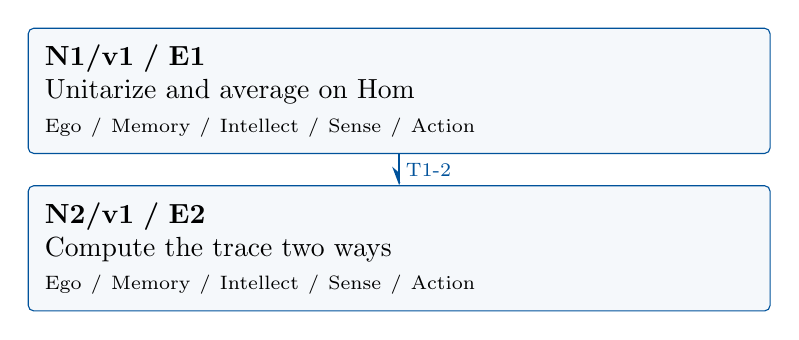
\begin{tikzpicture}[>=Stealth,x=1cm,y=1cm]

\node[mmnode,text width=9cm,minimum height=1.25cm] (N1) at (0,0.0) {\textbf{N1/v1 / E1}\\Unitarize and average on Hom\\{\scriptsize Ego / Memory / Intellect / Sense / Action}};

\node[mmnode,text width=9cm,minimum height=1.25cm] (N2) at (0,-2.0) {\textbf{N2/v1 / E2}\\Compute the trace two ways\\{\scriptsize Ego / Memory / Intellect / Sense / Action}};

\draw[mmproof] (N1.south) -- node[mmnote,right] {T1-2} (N2.north);

\end{tikzpicture}\end{center}

Each box is one mathematical agent containing all five faculties. Blue
arrows carry the versioned exports listed below. The layout gives a
reading order; only drawn arrows assert dependencies. Diagnostic repair
is separate from the proof DAG.

\subsection{Versioned evidence-transfer ledger}

\begingroup\small\linespread{1.05}\selectfont

\Needspace{5\baselineskip}\field{T1-2: N1/E1/v1 to N2}{\(P(A)=|G|^{-1}\sum_g g\cdot A\) is a projection onto
\(\operatorname{Hom}_G(V,W)\), and
\(\chi_V(g^{-1})=\overline{\chi_V(g)}\).}

\field{Receiving activity}{N2.1}

\field{Compatibility}{E1/v1 and the Hom dimension from RT-02. Check: Character conjugation
belongs on \(V\), the representation appearing with an inverse in the
Hom action.}

\endgroup

\clearpage\section{Agent roles and five-faculty activities}\begingroup\small\linespread{1.05}\selectfont\setlist{itemsep=1pt,topsep=2pt}

\subsection{N1/v1: Unitarize and average on Hom}

\field{Object and role}{Average positive forms to compare inverse traces with conjugates, and
average the Hom action to project onto invariants. \textbf{Local
obligation:} \(P(A)=|G|^{-1}\sum_g g\cdot A\) is a projection onto
\(\operatorname{Hom}_G(V,W)\), and
\(\chi_V(g^{-1})=\overline{\chi_V(g)}\).}

\field{Inputs}{\(\operatorname{Hom}_{\mathbb C}(V,W)\) with
\(g\cdot A=\rho_W(g)A\rho_V(g)^{-1}\).}

\mmfaculty{E}{Ego}{Publish E1/v1 only after establishing this obligation:
\(P(A)=|G|^{-1}\sum_g g\cdot A\) is a projection onto
\(\operatorname{Hom}_G(V,W)\), and
\(\chi_V(g^{-1})=\overline{\chi_V(g)}\).}

\mmfaculty{M}{Memory}{\(\operatorname{Hom}_{\mathbb C}(V,W)\) with
\(g\cdot A=\rho_W(g)A\rho_V(g)^{-1}\). Retain the stated assumptions and
import versions.}

\mmfaculty{I}{Intellect}{Average positive forms to compare inverse traces with conjugates, and
average the Hom action to project onto invariants.}

\mmfaculty{S}{Sense}{Every summand of the averaged form is positive on a nonzero vector;
finiteness makes the sum well defined.}

\mmfaculty{A}{Action}{Carry out activities N1.1--N1.2 below, retaining each calculation and
construction as evidence.}

\smallskip\noindent\textbf{Numbered mathematical activities}

\begin{enumerate}[label=N1.\arabic*,leftmargin=3.4em]

\item Start with a positive Hermitian form on each representation and replace
it by the sum \(\sum_g\langle\rho(g)v,\rho(g)w\rangle\). This remains
positive definite and is invariant by reindexing. In orthonormal bases
every \(\rho(g)\) is unitary, so the trace of its inverse is the complex
conjugate of its trace.

\item The conjugation formula defines a representation on Hom. Reindexing the
average shows \(P(A)\) is fixed by every group element. A fixed \(A\) is
unchanged by averaging; fixedness is exactly \(A\rho_V(g)=\rho_W(g)A\).
Therefore \(P^2=P\) and its image is the intertwiner space.

\end{enumerate}

\field{Export E1/v1}{\(P(A)=|G|^{-1}\sum_g g\cdot A\) is a projection onto
\(\operatorname{Hom}_G(V,W)\), and
\(\chi_V(g^{-1})=\overline{\chi_V(g)}\).}

\field{Acceptance gate}{Every summand of the averaged form is positive on a nonzero vector;
finiteness makes the sum well defined.}

\field{Targeted repair}{If an arbitrary initial inner product is assumed invariant, perform the
finite-group averaging before identifying inverse and conjugate traces.
Withhold this export and recheck its descendants after a versioned
correction.}

\clearpage

\subsection{N2/v1: Compute the trace two ways}

\field{Object and role}{Use a matrix-unit basis to factor the trace of left-right
multiplication. \textbf{Local obligation:} The normalized character
inner product equals \(\dim\operatorname{Hom}_G(V,W)\) and hence the
claimed Kronecker value.}

\field{Inputs}{E1/v1 and the Hom dimension from RT-02. Incoming proof exports: E1/v1 at
N2.1.}

\mmfaculty{E}{Ego}{Publish E2/v1 only after establishing this obligation: The normalized
character inner product equals \(\dim\operatorname{Hom}_G(V,W)\) and
hence the claimed Kronecker value.}

\mmfaculty{M}{Memory}{E1/v1 and the Hom dimension from RT-02. Incoming proof exports: E1/v1 at
N2.1. Retain the stated assumptions and import versions.}

\mmfaculty{I}{Intellect}{Use a matrix-unit basis to factor the trace of left-right
multiplication.}

\mmfaculty{S}{Sense}{Character conjugation belongs on \(V\), the representation appearing
with an inverse in the Hom action.}

\mmfaculty{A}{Action}{Carry out activities N2.1--N2.2 below, retaining each calculation and
construction as evidence.}

\smallskip\noindent\textbf{Numbered mathematical activities}

\begin{enumerate}[label=N2.\arabic*,leftmargin=3.4em]

\item For matrices \(B\) on \(W\) and \(C\) on \(V\), the diagonal coefficient
of \(A\mapsto BAC\) on the matrix unit \(E_{ij}\) is \(B_{ii}C_{jj}\).
Summing over \(i,j\) yields
\(\operatorname{tr}(A\mapsto BAC)=\operatorname{tr}B\operatorname{tr}C\).
Thus \(\operatorname{tr}P=|G|^{-1}\sum_g\chi_W(g)\chi_V(g^{-1})\).

\item Because \(P\) is idempotent, every \(A\) is the sum \(P(A)+(A-P(A))\)
from image and kernel, with zero intersection. Relative to that
decomposition, \(P\) has identity and zero blocks, so its trace is the
dimension of its image. E1 and RT-02 now give the desired zero or one,
and the inverse-trace identity gives the stated conjugated formula.

\end{enumerate}

\field{Export E2/v1}{The normalized character inner product equals
\(\dim\operatorname{Hom}_G(V,W)\) and hence the claimed Kronecker value.}

\field{Acceptance gate}{Character conjugation belongs on \(V\), the representation appearing
with an inverse in the Hom action.}

\field{Targeted repair}{If the inner product is written without conjugation, restore the inverse
representation in the Hom action and recompute its trace. Withhold this
export and recheck its descendants after a versioned correction.}

\endgroup\clearpage\section{Continuous mathematical proof}\label{sec:proof}

\subsection{N1 --- Unitarize and average on
Hom}\label{n1-unitarize-and-average-on-hom}

\begin{enumerate}
\def\labelenumi{\arabic{enumi}.}
\item
  \textbf{N1.1.} Start with a positive Hermitian form on each
  representation and replace it by the sum
  \(\sum_g\langle\rho(g)v,\rho(g)w\rangle\). This remains positive
  definite and is invariant by reindexing. In orthonormal bases every
  \(\rho(g)\) is unitary, so the trace of its inverse is the complex
  conjugate of its trace.
\item
  \textbf{N1.2.} The conjugation formula defines a representation on
  Hom. Reindexing the average shows \(P(A)\) is fixed by every group
  element. A fixed \(A\) is unchanged by averaging; fixedness is exactly
  \(A\rho_V(g)=\rho_W(g)A\). Therefore \(P^2=P\) and its image is the
  intertwiner space.
\end{enumerate}

\subsection{N2 --- Compute the trace two
ways}\label{n2-compute-the-trace-two-ways}

\begin{enumerate}
\def\labelenumi{\arabic{enumi}.}
\item
  \textbf{N2.1.} For matrices \(B\) on \(W\) and \(C\) on \(V\), the
  diagonal coefficient of \(A\mapsto BAC\) on the matrix unit \(E_{ij}\)
  is \(B_{ii}C_{jj}\). Summing over \(i,j\) yields
  \(\operatorname{tr}(A\mapsto BAC)=\operatorname{tr}B\operatorname{tr}C\).
  Thus \(\operatorname{tr}P=|G|^{-1}\sum_g\chi_W(g)\chi_V(g^{-1})\).
\item
  \textbf{N2.2.} Because \(P\) is idempotent, every \(A\) is the sum
  \(P(A)+(A-P(A))\) from image and kernel, with zero intersection.
  Relative to that decomposition, \(P\) has identity and zero blocks, so
  its trace is the dimension of its image. E1 and RT-02 now give the
  desired zero or one, and the inverse-trace identity gives the stated
  conjugated formula.
\end{enumerate}

\hfill$\square$

\section{Worked orchestration}

For \(C_3=\langle g\rangle\), let \(\chi_r(g^j)=\omega^{rj}\) for
\(r=0,1,2\). The inner product of \(\chi_r\) and \(\chi_s\) is
\((1+\omega^{s-r}+\omega^{2(s-r)})/3\). It is one when \(r=s\) and zero
otherwise by the geometric sum identity.

\subsection{Boundary and hypothesis audit}

Without complex conjugation, the supposed self-inner-product of
\(\chi_1\) for \(C_3\) would be \((1+\omega^2+\omega)/3=0\), although
the representation is nonzero irreducible. The conjugation is essential.

\section{Illustrative failure and repair}

The following is an authored diagnostic scenario. Changed assumptions
define a new contract; they do not retroactively prove the original
statement.

\subsection{Rejected argument, diagnosis, and correction}
\textbf{Rejected N2 calculation:}
\(\operatorname{tr}(g\cdot A)=\chi_V(g)\chi_W(g)\). \textbf{Sense
witness:} the zero self-inner-product above. \textbf{Diagnosis:} Action
lost the inverse matrix acting on the domain. \textbf{Repair:} retain
\(\rho_V(g)^{-1}\) in the matrix-unit calculation, then use unitarity to
conjugate its character. The corrected trace proves the original target;
recheck the final orthogonality export.

\subsection{Publication and reuse}
The corrected export retains its explicit assumptions. A hypothetical
revision receives a new version, and each consuming activity is
rechecked; this scenario is not a recorded runtime event. \textbf{Next
direction:} Derive multiplicities by taking inner products with
irreducible characters after complete reducibility is established.

\par\medskip\begingroup\small\linespread{1.0}\selectfont\noindent\textbf{Provenance.} This authored proof is complete relative to its declared imports. Reuse
each export with its assumptions, proof, and version. The original
Markdown remains available for comparison.
\par\endgroup

\par\smallskip\begingroup\small\linespread{1.0}\selectfont\noindent\textbf{Further reading.} \href{https://math.mit.edu/~etingof/reprbook.pdf}{Etingof and
collaborators, Introduction to Representation Theory}, sections on
representations, characters, and \(\mathfrak{sl}_2\);
\href{https://ocw.mit.edu/courses/18-745-lie-groups-and-lie-algebras-i-fall-2020/lists/lecture-notes/}{MIT
Lie Groups and Lie Algebras I lecture notes} for solvable Lie algebras.\par\endgroup

\end{document}
